\title{Self Organizing Maps (SOM)}
\label{chp:self-organizing-maps}
\author{George G. Cabral}
\institute{Department of Computing, Federal Rural University of Pernambuco, BR}
\maketitle



%\chapter{Optimization}

Self Organizing Maps (SOM) were initially introduced by Teuvo Kohonen \cite{kohonen:1982,khonen:1990} in the early 1980s inspired by the way the cerebral cortex handles sensory information, such as visual, olfactory and auditory information. The auditory cortex in the auditory system, for example, can be roughly represented as a surface (or map) so that different regions process different sound frequencies. In addition, nearby regions are responsible for processing similar frequencies. These concepts were successfully adapted from neuroscience to computer Artificial Neural Networks (ANNs) through the SOM networks. Among all types of ANNs, perhaps, the ANN architecture is the one which better resembles the human brain functioning. This chapter provides an introduction to SOM.

\section{An Overview of SOM's Mechanisms}

For practical purposes, a SOM network model uses as topological maps 2d or 3d grids such that each grid cell represents a neuron. Nevertheless, these maps can have different topological organizations. Figure \ref{fig:topologic} shows maps using two different topologies, squares and hexagons. In these maps, each unit (square or hexagon) represents an output neuron. %Figure \ref{fig:topologic} provides the insight for an important application of SOM networks, dimensionality reduction. 
 Most of real world problems lie in a high dimensional space. The map can be seen as a lower dimensional representation of the space. Finding a SOM model which maps the original space to a low dimensional space may result in, among the benefits, less data storage requirements, for example.

\begin{figure}[h]
\centering
\includegraphics[scale=0.08]{ "Part 3 - Learning Systems/Unsupervised Learning/Self-Organizing Maps/figs/maps"}
\caption{Examples of 2d maps. (left) squared map and (right) hexagonal map.}
\label{fig:topologic}
\end{figure}

Given a set of training examples $\mathcal{T} = \{\mathbf{x}^{(1)},\mathbf{x}^{(2)},\mathbf{x}^{(3)},\cdots,\mathbf{x}^{(N)}\}$, where each training example $\mathbf{x}^{(n)}$ is a $d$-dimensional vector, a training \textbf{epoch} consists in the presentation of the $n$ training examples to the classifier for learning purposes. Nevertheless, the whole training procedure takes several epochs, often, hundreds or more, i.e., the $n$ training examples are presented multiple times. The learning phase of a self organization involves 3 major concepts from neuroscience.
\vspace{0.2cm}

\noindent\textbf{Competition} As a training example \textbf{x}$^{(n)}$ is presented to the network, each neuron competes against the others in such a manner that the winner neuron is the neuron with its weights closer to \textbf{x}$^{(n)}$'s features. Notice that each neuron, therefore, has a set of $d$ weights associated to it (provided that $d$ is the number of problem features). The measure of how close a neuron is to a training example can be computed by the Euclidean distance between two examples (Equation \ref{eq:euclid_dist_som}).

\begin{equation}
    EuclidDist(\textbf{x}^{(i)},\textbf{z}) = \sqrt{(x^{(i)}_{1} - z_1)^{2} + (x^{(i)}_{2} - z_2)^{2} + \cdots + (x^{(i)}_j - z_j)^{2}}
    \label{eq:euclid_dist_som}
\end{equation}

\vspace{0.2cm}

\noindent\textbf{Cooperation} In the cerebral cortex, each received sensory stimulation results in a specific region which achieves a higher activation value - the winner neuron in the competition phase. Nevertheless, locations close to the winner region (the neighbourhood) are also activated by a smaller magnitude. This magnitude decreases and tends to zero as the regions get far from the winner neuron. In a SOM ANN, this concept is adapted by computing a neighbourhood to each neuron. Figure \ref{fig:cooperation} shows an example where the winner neuron (red) has its weights reinforced by a factor of 1, its closest neighbours (orange) have their weights reinforced by a factor of 0.5 and its indirect neighbours (yellow) have their weights reinforced by a factor of 0.25. 

\begin{figure}[h]
\centering
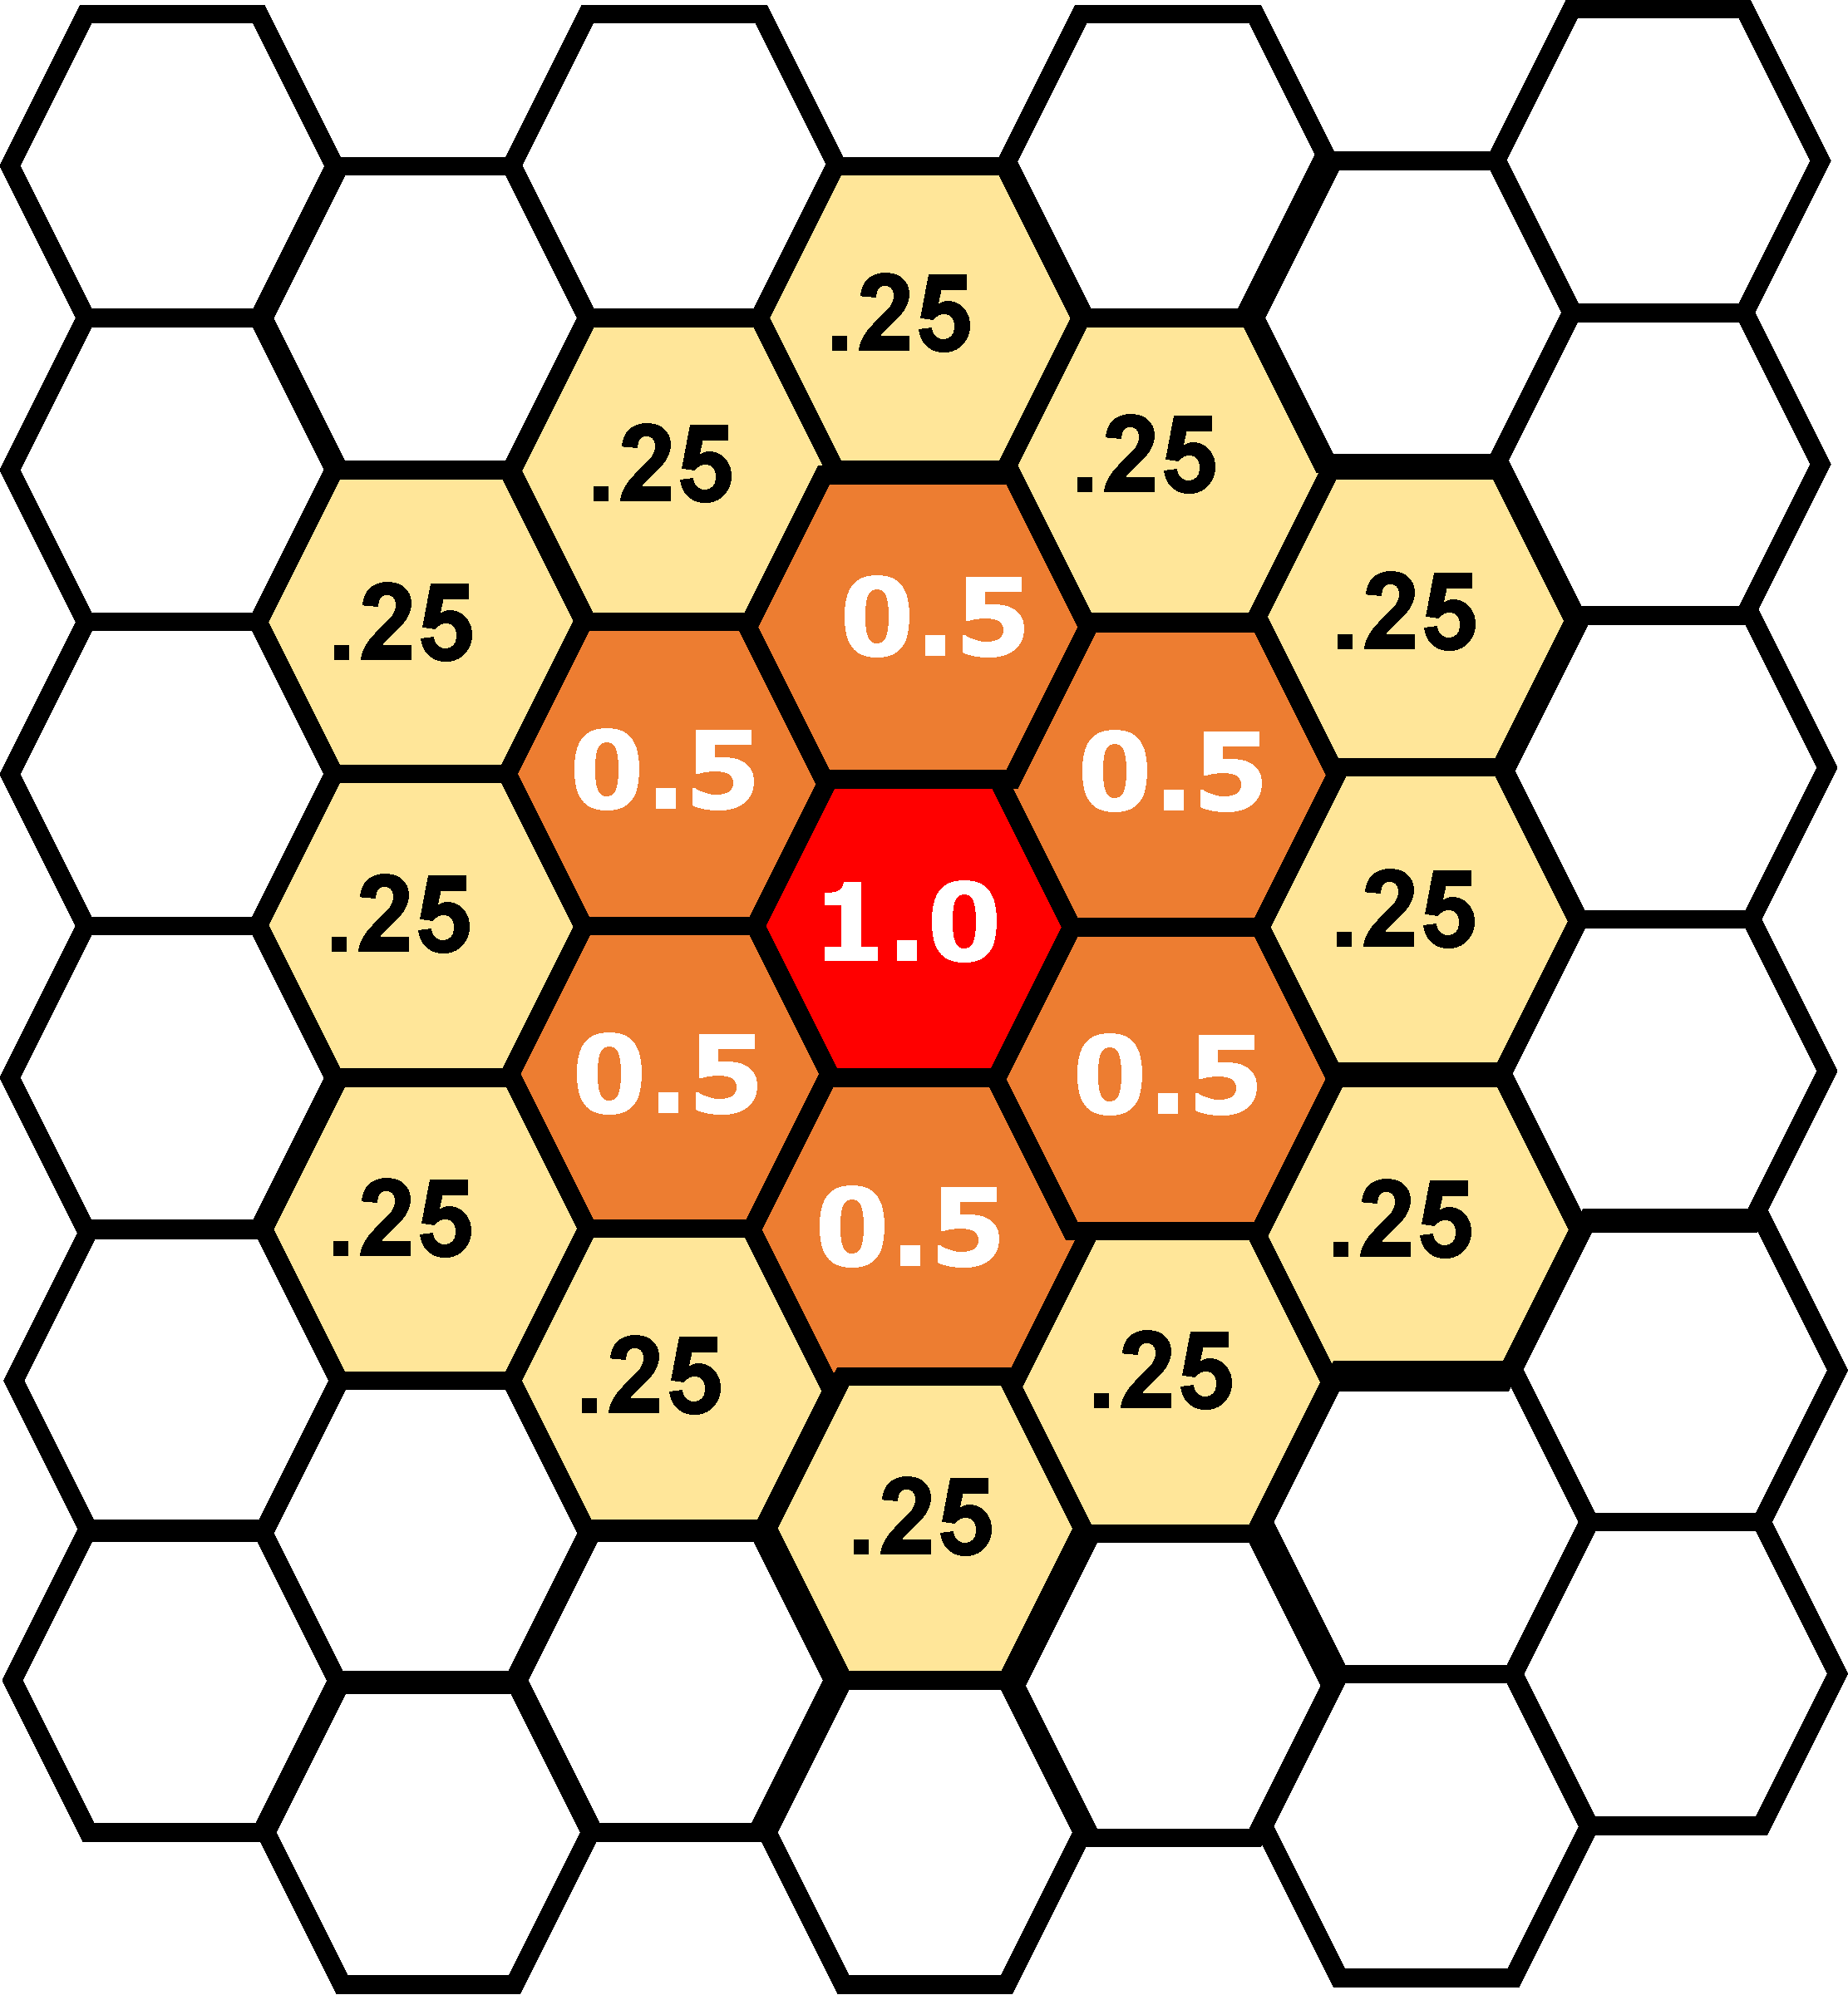
\includegraphics[scale=0.08]{"Part 3 - Learning Systems/Unsupervised Learning/Self-Organizing Maps/figs/cooperation.pdf"}
\caption{Example of neighbourhood and factors values of weight update according to the distance a of the neurons to a winner neuron.}
\label{fig:cooperation}
\end{figure}

A popular way to find the topological factor for weights update of the neighbour neurons is given by the use of a Gaussian function \cite{haykin:2009}. In order to rule the winner neuron neighbourhood, a function must possess two important properties: (1) to provide symmetric values from the winner neuron and (2) decrease monotonically as the distance from the winner neuron gets larger. The Gaussian function, presented in Equation \ref{eq:factor_update} has both properties. In Eq. \ref{eq:factor_update}, (i) $d_{a,b}$ consists in the distance between the winner neuron $a$ and its neighbour neuron $b$ and (ii) $\sigma_{t}$ is a decay factor at epoch $t$ that rules the coverage of the neighbourhood.  

\begin{equation}
    F_{a,b}(t) = exp(-d_{a,b}^2/2\sigma_{t}^2)
    \label{eq:factor_update}
\end{equation}

Ideally, as the time passes, $\sigma$ decreases, eventually, resulting in a neighbourhood comprising only the winner neuron. This happens because, initially, the SOM is coarsely learning the problem. As the time passes, the algorithm starts to refine the learning process to learn the problem's details. A common method to decrease $\sigma$ is given in Equation \ref{eq:sigma}. In Eq. \ref{eq:sigma}, $\tau_{1}$ is a constant and $\sigma_{0}$ is the first value assigned to $\sigma$.

\begin{equation}
    \sigma_{t} = \sigma_{0} exp(-t/\tau_{1}) \quad t = 0, 1, 2, 3,...
    \label{eq:sigma}
\end{equation}

For the multivariate case, a positive-definite covariance matrix must be defined. Similarly to the univariate case, shrinking the values in this matrix exponentially decreases the width of the neighbourhood function.  

Notice that the map topology may slightly influence the clusters' organizations. For example, in a square topology (Figure \ref{fig:topologic} (left)), a neuron may have up to eight direct neighbors that supposedly should be at the same distance to the winner neuron, however, the four neurons in the corner are more distant than the other four. In this case, choosing a small map (a map with few neurons) may lead to unsmooth separations between clusters. On the other hand, in the hexagon map (Figure \ref{fig:topologic} (right) and Figure \ref{fig:cooperation}), a winner neuron may have up to six closest neighbors all of them with the same distance to it. In this case, the topology allows a smother interaction among the winner neuron and its neighbors. 


\vspace{0.2cm}

\noindent\textbf{Adaptation} The adaptation (or learning) process takes place as the outputs neurons learn the problem making the topological map organized such that the clusters can be identified as the algorithm converges to a solution. As seen in the cooperation phase, not only the winner neuron moves toward a training example. Instead, the entire neighbourhood moves toward it. Once the winner neuron is found, its weights are updated according Equation \ref{eq:delta_weight}. The learning rate $\eta(t)$, as well as the neighbourhood size, also exponentially shrinks as the time passes. Therefore, one plausible way to shrink the learning rate is given by $\eta (t) = \eta_{0} (-t/\tau_{2})$, where $\tau_{2}$ is a constant and $\eta_{0}$ is the first value assigned to the learning rate.

\begin{equation}
    \Delta w_{j,i}(t) = \eta(t) \times F_{j,i}(t) \times (x_{i} - w_{j,i})
    \label{eq:delta_weight}
\end{equation}

\vspace{0.2cm}


In short and recapping, in practice, (i) during the \textbf{competition phase} a winner neuron (\textbf{c}) is found, (ii) in the \textbf{cooperation phase} a set of \textbf{c}'s neighbors in the topological map is defined and (iii) in the \textbf{adaptation phase} the weights of the winner neuron and its neighbors are adjusted.

\section{The Self Organizing Map Algorithm}
\label{sec:som}

The vast majority of the works define the SOM topology as containing only the input and output layers. The input layer, as most of the ANNs, acts as sensors so that the number of neurons is the same as the number of features of the problem. Therefore, the domain of the input layer is $\mathbb{R}^{d}$, where $d$ is the number of features of the problem. The output layer (or the Kohonen layer) is usually a 2-dimensional map (Figure \ref{fig:architecuture}) where each cell represents a different neuron. The input layer is connected to each output neuron such that the number of connections is given by $d \times j$, where $j$ is the number of output neurons. Figure \ref{fig:architecuture} depicts an example of SOM architecture where $j = 88$. The input layer, is formed by $d$ neurons fully connected to each output neuron and each connection between input neuron $i$ and output neuron $j$ has an associated weight $w_{i}^{(j)}$. In Figure \ref{fig:architecuture}, the connections between the input layer and the output neuron 1 (one) are highlighted in red.

\begin{figure}[h!]
\centering
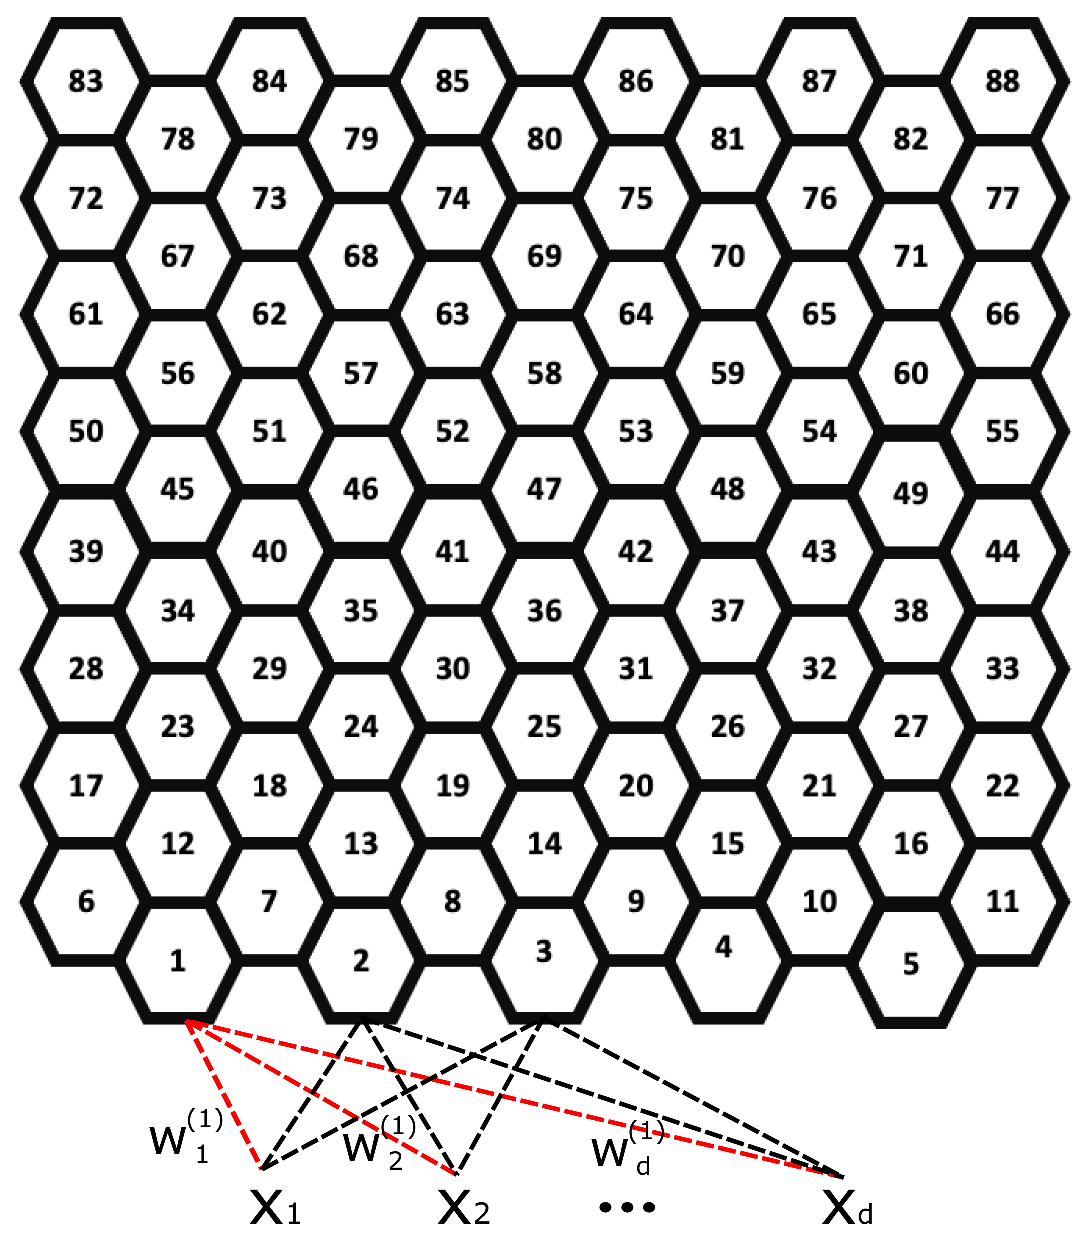
\includegraphics[scale=0.35]{"Part 3 - Learning Systems/Unsupervised Learning/Self-Organizing Maps/figs/arquitetura.pdf"}
\vspace{-3cm}
\caption{Partial example of SOM architecture. The connections between the input layer and the output neuron 1 are highlighted in red.}
\label{fig:architecuture}
\end{figure}



\begin{algorithm}[h!]
    \caption{Self Organizing Map}
    
    Parameters: output map containing $j$ neurons and $d \times j$ connections with respective weights ($w_{d}^{(j)}$) between input and output layers, neighborhood function $F$, $\tau_1$, $\tau_2$, $\eta_{0}$, $n\_epochs$, training set $\mathcal{T}$, $\theta$  
    
    Output: SOM model with proper weights between input and output layers
    
    \begin{algorithmic}[1] 
    
    \STATE Set a random value for each of the $j \times d$ weights at each connection between the input and output layers. These values must be in the same interval of the feature values in $\mathcal{T}$.
    
    \FOR{$t \in \{1 \cdots n\_epochs\}$}
    
    \FOR{$\mathbf{x}^{(i)} \in \mathcal{T}$}
    
      \STATE Given $\mathbf{x}^{(i)}$, find the winner neuron $c$ 
      
      \FOR{$k \in \{1 \cdots d\}$}
      
      \STATE $\Delta w_{k}^{(c)}(t) = \eta(t) \times EuclidDist(x_{k}^{(i)}, w_{k}^{(c)})$
      
      \STATE $w_{k}^{(c)} = w_{k}^{(c)} + \Delta w_{k}^{(c)}(t)$
      
      \ENDFOR
      
      
      
      \FOR{each neighbor $neigh$ of $c$}
        
        \FOR{$k \in \{1 \cdots d\}$}
        
        \STATE $\Delta w_{k}^{(neigh)}(t) = \eta(t) \times F_{c,neigh}(t) \times EuclidDist(x_{k}^{(i)}, w_{k}^{(neigh)})$
        
        \STATE $w_{k}^{(neigh)} = w_{k}^{(neigh)} + \Delta w_{k}^{(neigh)}(t)$ 
        
        \ENDFOR
        
        
      \ENDFOR
    
    \ENDFOR
    
    \COMMENT{$\sigma_{t}$ is used in the neighborhood function $F_{x,y}(t)$}
    \STATE $\sigma_{t+1} = \sigma_{t} exp(-t/\tau_{1})$ 
    
    \STATE $\eta (t+1) = \eta_{t} (-t/\tau_{2})$
    
    \ENDFOR %epochs
    
    \end{algorithmic}


\label{alg:som}
    
\end{algorithm}

Algorithm \ref{alg:som} depicts the operation sequence of a SOM neural network for a problem containing $d$ features and $j$ output neurons. Initially (line 1), all the weights for the connections among the input neurons and output neurons are randomly set. In line 4, a training example \textbf{x}$^{(i)}$ is presented and the closest neuron to it in the map ($c$) is chosen as winner. The weights of $c$ then 
``move toward'' \textbf{x}$^{(i)}$ considering the learning rate $\eta(t)$ (lines 6 and 7). The same adjustment happens to the weights of the neighbors of $c$ in the map, however, in this case the adjustment is ruled by an additional distance factor computed by the neighborhood function $F_{x,y}(t)$ so that neighbors closer to $c$ have their weights strongly updated (lines 11 and 12). Lines 16 and 17 are responsible for the update of parameters that affect the fine convergence of the algorithm in later epochs. 

% \begin{enumerate}
%     \item Empirically set the output topology and assign values to $\eta_{0}$, $\tau_{1}$ and $\tau_{2}$. Additionally define the parameters of the neighbourhood function.
%     \item Set a random value for each of the $j \times n$ weights at each connection between the input and output layers. These values must be in the same interval of the feature values in $\mathcal{T}$.
%     \item Compute the distances between a random training example $x^{(a)}$ and each neuron in the output layer and find the closest one ($b$) (i.e., the winner neuron). 
%     \begin{enumerate}
%         \item Update the weights of $b$ as follows: $\Delta w_{i}^{(b)}(t) = \eta(t) \times 1 \times (x_{i}^{(a)} - w_{i}^{(b)})$
%         \item For each $b$'s neighbour $z$ neuron where $F_{(b,z)}(t) > \theta$: $\Delta w_{i}^{(z)}(t) = \eta(t) \times F_{b,z}(t) \times (x_{i}^{(a)} - w_{i}^{(z)})$
%     \end{enumerate}
%     \item Update $\sigma(t)$ and $\eta(t)$.
%     \item While the pre-defined maximum number of epochs hasn't been reached go to the step 3, otherwise, return the trained model.
% \end{enumerate}


At the end of the training phase, it is expected that output neurons in a same topological region represent a cluster (or class). In particular, examples that are similar to each other are mapped to the same or nearby regions of the topological map.

%As seen in the previous paragraphs, the SOM is formed by (i) an input layer with the same size as the number of features of the problem and (ii) an 2d or 3d output layer. Each output neuron is fully connected to the input layer. Furthermore, the topological location of the output neurons is key such that at the end of the training phase, output neurons in a same topological region represent a cluster (or class). 

\subsection{Example of the Algorithm Execution}
\label{sec:algorithmExecution}

In order to provide a comprehensive understanding of the canonical SOM algorithm, Figure \ref{fig:trset} presents a 3-dimensional dataset containing 16 colors in the RGB format which will be learned so that the main stpdf of the algorithm can be shown. Notice that the clustering algorithms assume that there is redundant information in the training set, therefore, we inserted variations of the dominant colors blue, green, black and brown in the dataset. 

\begin{figure}[h!]
\centering
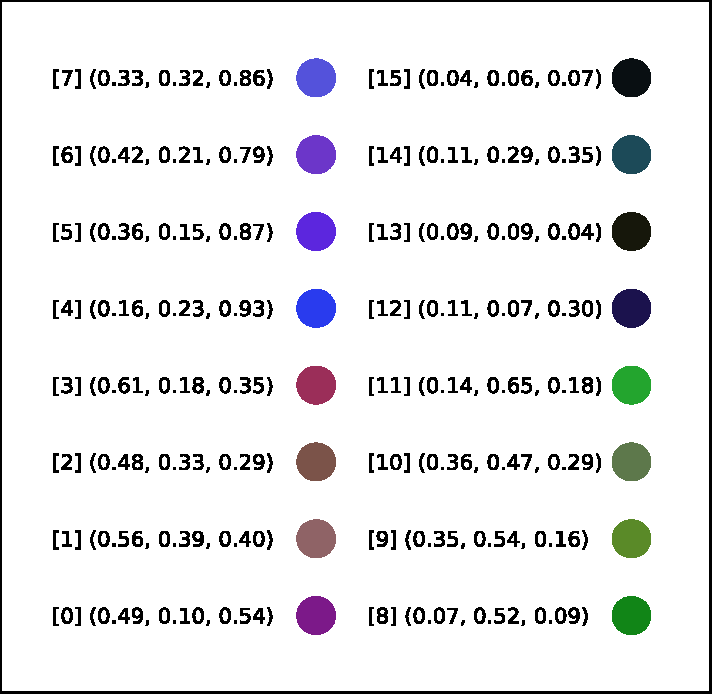
\includegraphics[scale=0.6]{"Part 3 - Learning Systems/Unsupervised Learning/Self-Organizing Maps/figs/trainingSet.pdf"}
\caption{Training set containing 16 RGB colors where each color component is normalized between 0 and 1 and the presentation order of the examples is indexed in square brackets.}
\label{fig:trset}
\end{figure}

Initially, the topological map must be defined. For this example a (20, 20) matrix where each neuron is 1 unit distant from its nearest neighbor in the same row (or column) was used. In the sequel, for each neuron $b$, each connection's weight $w_{k}^{(b)}$ (where $k$ varies from 0 to 2) is randomly assigned between 0 and 1. In other words, for this problem we can say that, initially, each output neuron will be associated to a random RGB color (Figure \ref{fig:execution} a)).

The algorithm parameters were as follows:
\begin{itemize}
    \item $\eta_{0} = 0.5$ (initial learning rate)
    \item $\theta = 0.05$ (threshold for which the neighborhood function is considered)
    \item $\sum = [1.5, 0.0; 0.0, 1.5]$ (covariance matrix for defining the Gaussian neighborhood function)
    \item For this example, $\tau_{1}$ and $\tau_2$ weren't used since the learning rate and neighbourhood size weren't decreased. 
\end{itemize}

Notice that some of these parameters values are unlikely to be used in practice (as the initial learning rate value of 0.5, for example), but in this case, they were chosen for illustration purposes.

The very first step of the algorithm searches for the nearest neighbor (lets call it \textit{b}) in the map of the training example of index [0] in Figure \ref{fig:trset} (lets call it \textit{a}), i.e., (0.49, 0.10, 0.54). The nearest neighbor output neuron in the map is the neuron with closest weights, in this case (0.46 0.31 0.59). Therefore, the new weights of \textit{b} are computed as follows:

\vspace{0.2cm}

\noindent $W_{b,0}(t) = W_{b,0}(t-1) +  \eta(t) \times F_{a,b}(t) \times (x_{0}^{(a)} - w_{0}^{(b)}) = 0.46 + 0.5 * 1 * (0.49 - 0.46)$

\vspace{0.2cm}

\noindent $W_{b,1}(t) = W_{b,1}(t-1) +  \eta(t) \times F_{a,b}(t) \times (x_{1}^{(a)} - w_{1}^{(b)}) = 0.46 + 0.5 * 1 * (0.10 - 0.31)$

\vspace{0.2cm}

\noindent $W_{b,2}(t) = W_{b,2}(t-1) +  \eta(t) \times F_{a,b}(t) \times (x_{2}^{(a)} - w_{2}^{(b)}) = 0.46 + 0.5 * 1 * (0.54 - 0.59)$

\vspace{0.2cm}

In the sequel, all neighbours neurons, i.e., the neurons whose the scaled neighbourhood function yields a larger value than $\theta$ have theirs weights adjusted accordingly this value. 

This procedure is repeated for each training example in order to complete a training epoch. The total number of epochs is defined by the practitioner. 

Figure \ref{fig:execution} depicts part of the evolution of the algorithm computation above presented in terms of the topological map. Figure \ref{fig:execution} a) shows the initial state of the topological map where each neuron represents a random RGB color. In Figure \ref{fig:execution} b), the winner neuron of the 1st epoch and 1st training iteration (\textit{b}) with weights (0.46 0.31 0.59), has its neighbourhood defined (crosses points) so that for each neighbour $z$ $F_{b,z}(t) > \theta$. Notice that the winner neuron is computed according the neuron weights and the neighbourhood is defined based on the topological distance in the map to the winner neuron. Figure \ref{fig:execution} c) and d) also refer to the first epoch shows the computation for the winner neurons for the training set examples positioned at indexes 4 and 11. Figure \ref{fig:execution} e) presents an example of computation for the 6th epoch. In this stage is already possible to notice some clusters. Figure \ref{fig:execution} f) represents the topological map at 20th epoch. At this stage, the map is close to the convergence due to the small number of examples in the training set.


\begin{figure}[h!]
\centering
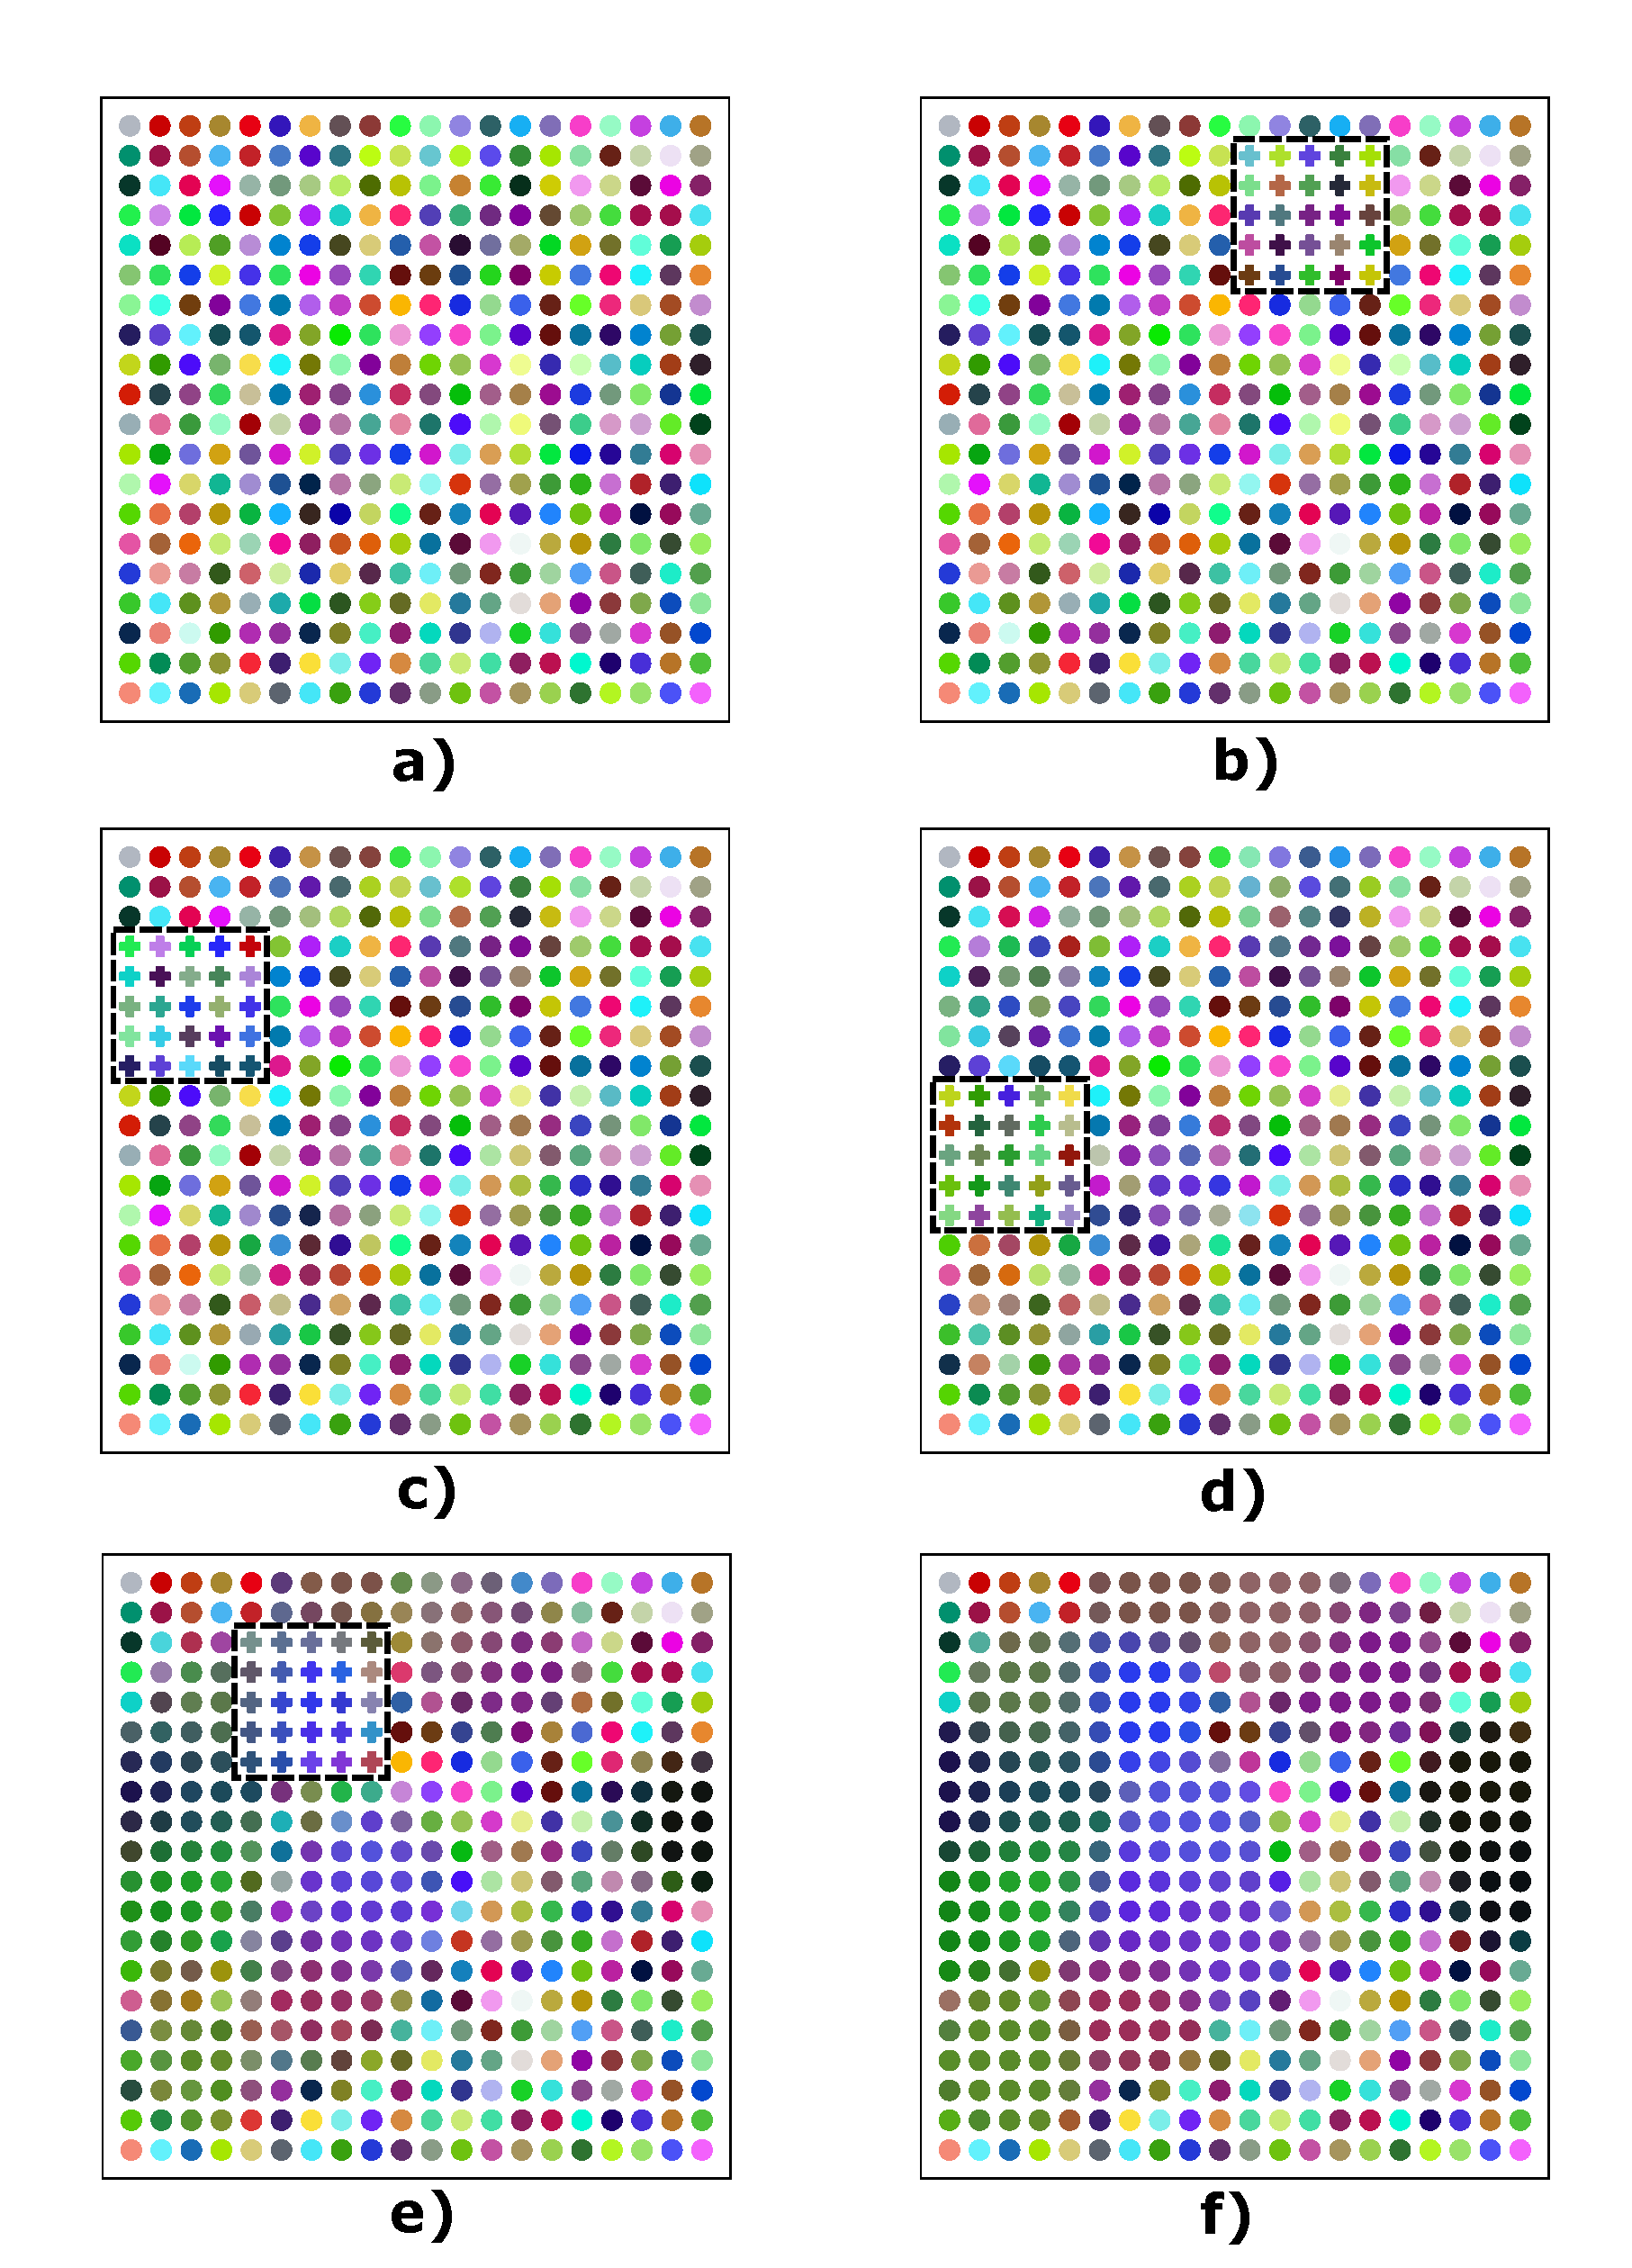
\includegraphics[scale=0.35]{"Part 3 - Learning Systems/Unsupervised Learning/Self-Organizing Maps/figs/SOM_Exec.pdf"}
\caption{a) Original random topological map; b) Epoch 0 - training example [0] neighbourhood after their weights' updates; c) Epoch 0 - training example at position 4's  neighbourhood after their weights' updates; d) Epoch 0 - training example at position 11's neighbourhood after their weights' updates; e) Epoch 5 - training example at position 4's neighbourhood after their weights' updates; f) Map status at epoch 20.}
\label{fig:execution}
\end{figure}



\vspace{0.2cm}

\noindent \textbf{Implementation Issues}

\vspace{0.2cm}

The PDF defined by the vector $b$ and $\sum$ is comprised in the interval ($0$, $r$), where $0$ is located at the infinite and $r$ is the largest value located at the mean $b$. For the current implementation, $r$ was scaled between 0 and 1. This explains the value 1 for the neighbourhood function in the previous weights adjustments.

Particularly for this illustration example, the small number of examples in the training set combined to the small variation in these examples caused, from a specific epoch, the winner neurons converge to the same neurons again and again. This explains some untouched areas in the map, such as the last row. 

% \noindent \textbf{Algorithm execution:}

% \vspace{0.2cm}




\section{Growing Self Organizing Map (GSOM) - A Dynamic version of SOM}

The GSOM was initially developed by Alahakoon and Srinivasan \cite{Alahakoon:2000} who claimed that their method had significant advantages for knowledge discovery over the original one. The main difference between both methods consists in a \textit{growing} topological map introduced in the GSOM. Furthermore, given the growing feature of the GSOM, its spreading factor enables the practitioner to track hierarchical aspect of the clusters, i.e., one can find the path from a finer cluster to a higher level cluster.  

The following high level stpdf depicts the GSOM algorithm:

\begin{enumerate}
    \item Initialization Phase
    \begin{enumerate}
        \item Randomly assign weights to, usually, 4 neurons connected in a 2d grid.
        \item Compute the Growth Threshold (GT) based on pre-defined parameters. 
    \end{enumerate}
    \item Growing Phase 
    \begin{enumerate}
        \item Present a training example to the network.
        \item Find the winner neuron, similar to the original SOM.
        \item Update weights values of the winner neuron and its neighbors as well as in the original SOM method
        \item The difference between the weights and the training example will be used as an error to be accumulated in the winner neuron as its total error (TE)
        \item If TE $>$ GT and the winner neuron is a boundary neuron, grow it (i.e., place new neurons in free positions in the neighbourhood of the current neuron. For example, above or at right.). Otherwise, distribute its weights to the neighbors of the current neuron.
        \item Initialize the new nodes weights to match the current neighbourhood
        \item Reset the learning rate to its starting value
        \item Repeat stpdf a. to g.
    \end{enumerate}
    \item Smoothing phase
    \begin{enumerate}
        \item Decrease the learning rate and fix a small neighbourhood.
        \item Repeat weights adaptation as in the growing phase.
    \end{enumerate}
\end{enumerate}

Amongst the advantages of the GSOM over the SOM are its capability to represent more complex topological maps and the possibility to discover hierarchical relationships, as previously mentioned.

This is a high level description of the GSOM. Many details, such as new nodes growth situations, new node weights assignment and neighborhood definition, were uncovered since this is not the aim of this text. For more details, the introductory paper \cite{Alahakoon:2000} as well as available implementations on the web can be helpful.


\section{Applications}

Virtually, SOM networks can be applied to any knowledge area. Nevertheless, some of them have been particularly benefited from its potential.

\subsection{Dimensionality Reduction}

Dimensionality reduction consists in transforming a problem from a high dimensional space to a low dimensional space. Among other, this enable us to: (i) better visualize relationships among the categories of the problem; (ii) reduce the noise effect on the data; (iii) identify clusters; and (iv) create models which serve as filters to reduce the data storage. 

Dimensionality reduction is a natural application of Self Organizing Maps given that transforming a n-dimensional problem to a 2d or 3d map explicitly reduces the original problem data dimension. The popularity of SOMs networks amongst different science fields caused them to be subject of studies for the feature reduction for a number of different problems \cite{pmid:24575660}\cite{Pratiwi2012TheUO}\cite{kutlu}\cite{liu}.



\subsection{Surface Reconstruction}

Reconstructing the surface of an object based on a set of examples structured or not is a common problem in many fields such as medicine \cite{Satava}, Arts \cite{974519} and manufacturing \cite{Bernardini}. The idea is to reproduce the original shape based on a partial set of examples, i.e., these examples may not be able to represent missing parts of the shape. SOMs can generate a map that is close to the original shape given a training set provided with the spatial coordinates of the points \cite{4371248}. Commonly, reconstruction process of methods based on self organizing maps use randomly sampled 3d points as training data for the learning algorithm where the mesh vertices correspond to the output nodes of the map \cite{4371248}. Some examples of images reconstructed from 3d points can be found at: \url{https://github.com/alecjacobson/common-3d-test-models}. Some examples of works that use SOMs or its variations for surface reconstruction are: \cite{Yu99surfacereconstruction}, \cite{1380023} and \cite{4371248}

\subsection{Image Segmentation}

Image segmentation consists in identifying the boundaries (lines, curves, etc.) of the objects present in an image. Some goals behind this are to reduce the amount of information in order to better track video objects, identify areas of interest, etc.. As an example, in a image containing a group of persons, imagine that you want to identify faces so that from these faces you can eventually find some specific person. With this aim, we may need to separate the image in many regions such that pixels in the same region share similar characteristics, as color values, and there are no abrupt changes in these characteristics inside the same region. For this task, SOMs can act as an intermediary step \cite{somImSeg1}\cite{somImSeg2}\cite{somImSeg3}\cite{somImSeg4}. Figure \ref{fig:imgSeg} depicts an example that can be used to segment images captured by an autonomous car sensor, for example. 


\begin{figure}[!h]
\centering
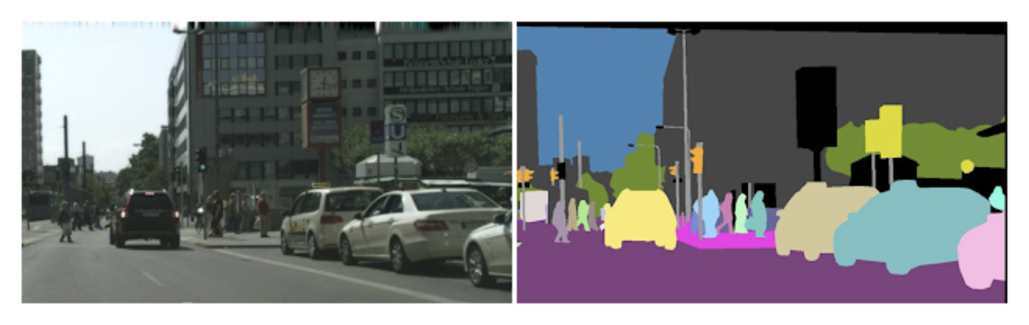
\includegraphics[scale=0.55]{ "Part 3 - Learning Systems/Unsupervised Learning/Self-Organizing Maps/figs/imageSeg.pdf"}
\caption{Segmentation for object identification in a traffic image. Source: Cityscapes Dataset \cite{Cordts2016Cityscapes} \url{https://www.cityscapes-dataset.com/}.}
\label{fig:imgSeg}
\end{figure}


\subsection{Text Mining}

Clustering documents is one of the most important text mining research areas \cite{txtmin1}\cite{txtmin2}\cite{txtmin3}. Even though some details are lost in this simplification, other information arise and, thus, we can observe the data from a macro point of view \cite{Liu12}. Liu et al. \cite{Liu12} also pointed out that text clustering can also act as a pre-processing step for some natural language processing applications, e.g., automatic summarization, user preference mining, or be used to improve text classification results. 

\subsection{Speech Recognition}

Speech recognition is an area that can vastly be benefited by self organizing maps, particularly by dynamic SOMs \cite{sp1}\cite{sp2}\cite{sp3}. For example, customer services of big companies rely on automatic speech recognition to actuate on call centers in order to understand \textit{yes} or \textit{no} questions and diminish the need of human interaction. In addition, a number of electronic devices also use voice recognition tasks to translate voice commands to machine entries. These type of applications can employ Self Organizing Maps for the end of the application, e.g., for classify a voice signal as \textit{yes} or \textit{no}, or as an intermediary procedure, e.g., for pre-processing voice signals in categories. 

\section{Strengths and Weaknesses of SOM networks}

One the main advantages of SOM networks it's that it can easily represent similarities in the data without the need of a complex fine tuning of the classifier's parameters (i.e., finding the output neurons' topology and the learning rate is not a complex task). The simplicity of the algorithm may be also seen as an advantage since knowing how the method behaves provides the practitioner with ability to customize it to domain specific problems. 

Among the disadvantages of SOM networks it is the necessity of a large amount of data to operate. Sufficient data is a necessary condition for most of the unsupervised learning algorithms to perform well, nevertheless, for SOM networks, depending on the training parameters and as the number of training epochs increase a small cluster may be forgotten in the case of a class imbalanced problem, for example. Another issue is the fact that it may converge to a map containing two similar clusters distant from each other according to the number of trained epochs and learning rate values. In addition, it may not perform well for categorical data as well. Still, a large number of SOM variations are available to address the original SOM's issues. 

\section{Summary}

The Self Organizing Map ANN, also called Kohonen map, is a simple, yet, effective clustering algorithm. Different from other neural networks SOM networks use competitive learning instead of error correction for training purposes. In comparison to other clustering algorithms, it does not require much \textit{apriori} knowledge of the data, such as the number of clusters or the cluster's density, to operate. 

Given the arrangement presented in the topological map it is intuitive the use of SOM networks, in addition to clustering, also for dimensionality reduction in the data. Therefore, many of the applications of SOM networks involve data representation. This chapter has shown some popular SOM applications, however, as the number of SOM variants grow, the number of problems tackled by this family of algorithms multiplies.  

\section{Exercises}

All resources necessary for the exact reproduction of the experiments in the exercises below are provided in a python notebook available at: \url{https://colab.research.google.com/drive/1_1ukwihWCfgK7288sX2FH9zLAot_s-ft?usp=sharing}. Alternatively, you can also access them at the code folder within the folder of this chapter of the book in its git repo: \url{https://github.com/ieee-cis/IEEE-CIS-Open-Access-Book-Volume-1}.

\begin{enumerate}
    \item Given the dataset of Figure \ref{fig:trset}, instantiate a (2,2) topological map and execute one training epoch without considering the neighborhood function.
    \item For the training set of Figure \ref{fig:trset} and a (10,10) topological map compute:
    \begin{enumerate}
        \item The neighborhood function for each neighbor of the winner neuron of the first training example given the covariance matrix provided in Section \ref{sec:algorithmExecution}. 
        \item Change the values of the covariance matrix and compute again the neighborhood function for each neighbor of the winner neuron of the first training example.
        \item Plot the bidimensional Gaussian function generated by each examined covariance matrix. 
    \end{enumerate}
    \item Change the provided code for the example in Section \ref{sec:algorithmExecution} to handle a dataset containing 1000 examples of different shades of colors red, green and blue. Change also the map to a 50 x 50 map. Introduce the use of parameters $\tau_1$ and $\tau_2$ by changing the parameter of the neighborhood function and the number of epochs such that the algorithm perform a refinement at later eopchs. 
    \item Explain the main differences between the clustering algorithms k-means and SOM.
    
\end{enumerate}


\bibliographystyle{unsrt}
\bibliography{bibliography}
